\documentclass[11pt,letterpaper]{article}

\usepackage[margin=1in]{geometry}
\usepackage{graphicx}
\usepackage{booktabs}
\usepackage{tabularx}
\usepackage[hidelinks]{hyperref}
\usepackage{listings}
\usepackage{xcolor}
\usepackage{lmodern}

\lstset{
    basicstyle=\ttfamily\small,
    backgroundcolor=\color{gray!8},
    frame=single,
    breaklines=true,
    numbers=left,
    numberstyle=\tiny,
    showstringspaces=false,
    tabsize=4
}


\lstdefinestyle{evidence}{
    basicstyle=\ttfamily\fontsize{7}{8.4}\selectfont,
    backgroundcolor=\color{gray!5},
    numbers=none,
    frame=single,
    breaklines=true,
    columns=fullflexible,
    keepspaces=true,
    showstringspaces=false,
    captionpos=b
}
\lstdefinestyle{evidencefull}{
    style=evidence,
    basicstyle=\ttfamily\fontsize{6.5}{7.8}\selectfont
}
% Resolve assets when building from documentation/ or the repository root.
\graphicspath{{../images/}{images/}}
\IfFileExists{evidence/run-59ewk1/01-silver.txt}{
    \newcommand{\reportdir}{.}
}{
    \newcommand{\reportdir}{documentation}
}
\newcommand{\captureroot}{\reportdir/evidence/run-59ewk1}
\newcommand{\validationroot}{\reportdir/evidence/validation-1AYnOc}

% Based on the Report requirements in Team_Project (4).pdf.
% Main report: at most eight pages. An appendix is permitted if needed.
% Submit the report PDF with the final code as a zip file.
% Comments indicate material still to be completed.

\title{CPS 853 Team Project Report}
\author{Hunter Huchenski} % Add team members' names.
\date{}

\begin{document}

\maketitle

\section{Design}
% 2 marks.

\subsection{Architecture Diagram}
Figure~\ref{fig:architecture} shows the implemented pipeline and its persistent outputs.
\begin{figure}[p]
    \centering
    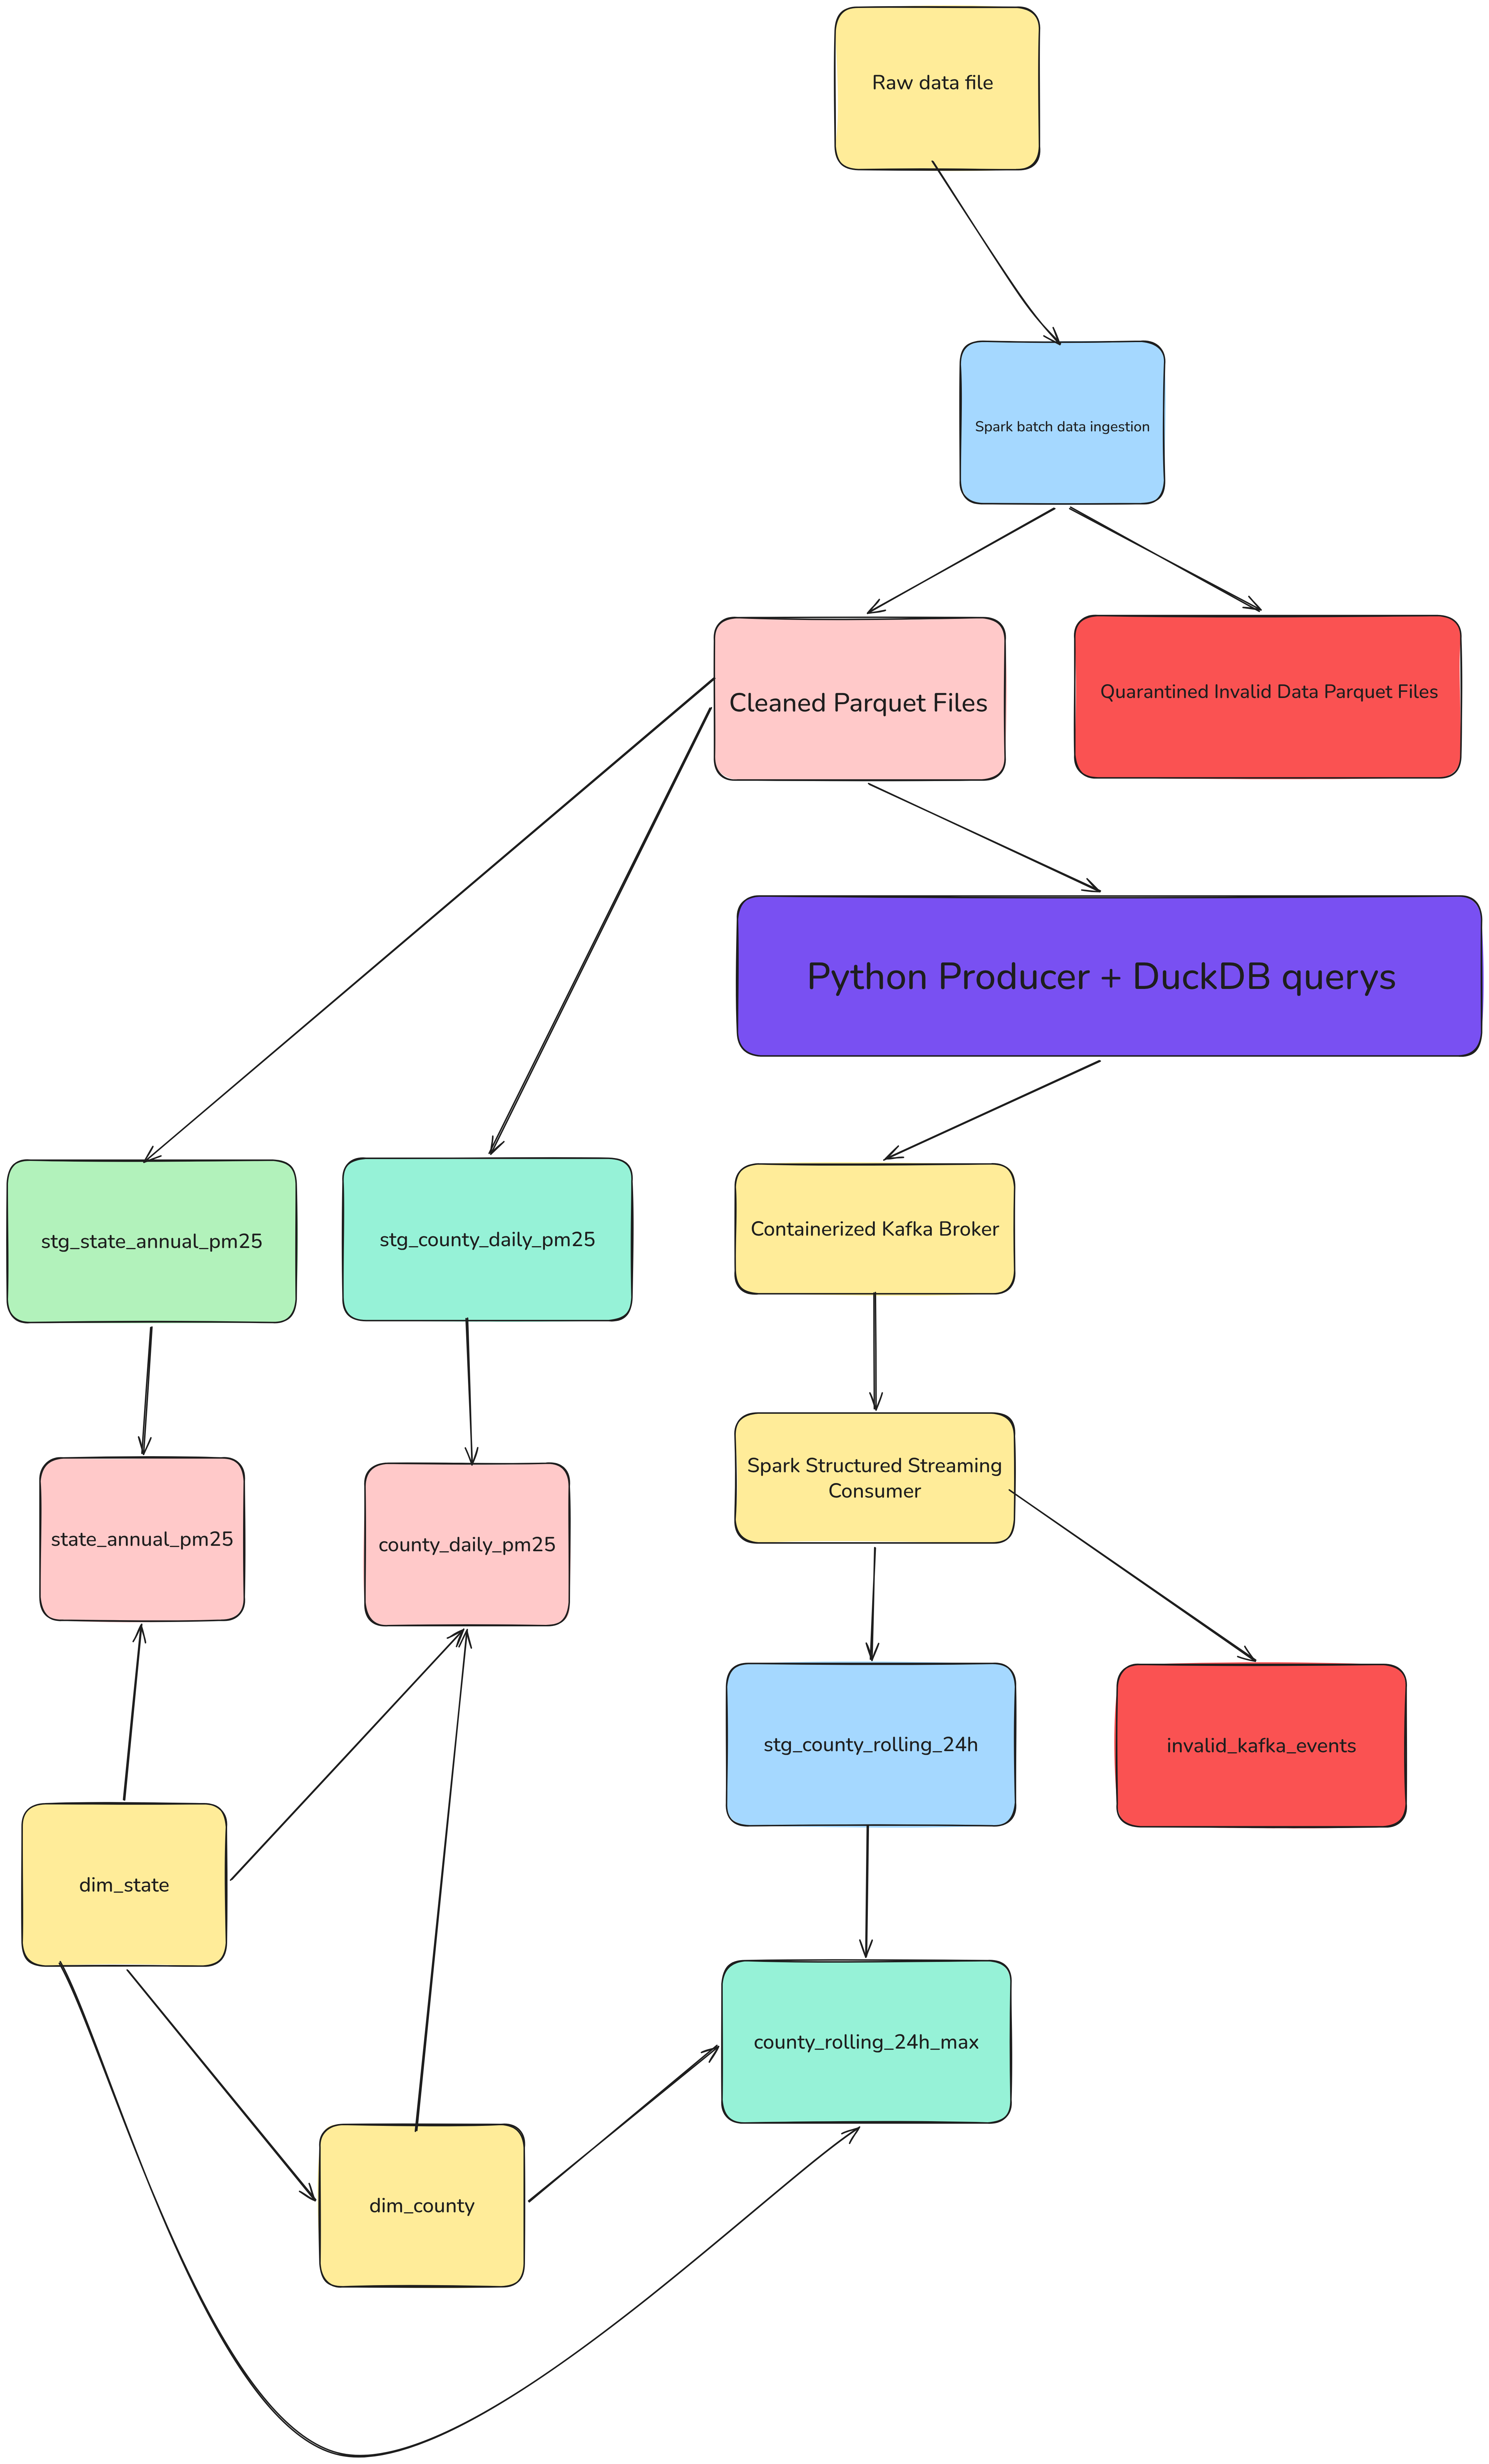
\includegraphics[
        width=\textwidth,
        height=0.85\textheight,
        keepaspectratio
    ]{architecture.png}
    \caption{System architecture: batch and Kafka streaming paths, quarantine storage, and PostgreSQL serving tables.}
    \label{fig:architecture}
\end{figure}

\subsection{Design Overview}
The data platform is as follows. Raw data is input into a spark batch processing job that takes a raw data-frame and separates valid and invalid rows. Valid rows are written to parquet files corresponding to a clean silver layer of data. The silver layer is where naming conventions are standardized and data-types are set, it reflects data that can be most easily used for aggregations and other processing activities. 

Invalid rows from this step are written in their raw form to parquet files that represent quarantined data. From this stage we move in two directions, one to the streaming pipeline and one to the gold batch processing pipeline. 

The gold pipeline runs the aggregations for the first two queries and then also writes these aggregations to 4 tables. Each final table has a staging table that all data is written to first. Once data is in the staging table via an append workflow we can run an upsert from the staging table into the final tables. 

The streaming pipeline starts with a producer that uses Duck-db to select rows from the parquet files, serialize these rows into messages with keys that correspond to a conjunction of the data's state-code and county-code. These messages are published to a kafka broker running on a docker container. 

The consumer of this data is built using spark structured streaming. Our spark consumer reads data in micro-batches, and checks if data is correctly shaped. If it is not then it is written to an quarantine table for invalid data. Valid data is used to calculate rolling 24 hour windows corresponding to rolling averages of pollution. The process is for each micro-batch calculate windows and then publish them to a staging table. Once all batches are processed we then run a sql query that extracts max daily windows from the staging table and publishes them to our final aggregates table.

Our SQL database can be queried with three main tables to get answers to the three questions. We also created two dimension tables, one for counties and one for states + counties that allows us to map state codes and county codes from the aggregates tables to their names. This allowed us to not have to store name data with every row of the aggregates tables.


\subsection{Database Choice and Alternative}
% Compare the selected database with one alternative and justify the choice.
The choice of persistent storage was PostgreSQL. The reasoning was that I wanted the serving layer to be a standard data warehouse. I used dimensional tables for states and counties so I could make use of star schemas to join fact tables (the data used for aggregations) and dimensions (the data used for joins to make outputs readable). Since the majority of the work was done by spark, the serving layer storage needs are not computationally heavy. This means that we could have used MongoDB, or basically any other SQL database, however since I wanted to create a data warehouse with a star schema based approach, SQL was the best choice for my design.

\subsection{Changes Since the Proposal}
% Describe any changes and give the reason for each.
The main change since the proposal is the third question. I changed it to use a sliding window calculation so I could make use of the event driven nature of Kafka. The new question was “Which U.S. counties experienced the highest average PM2.5 concentrations over any consecutive 24-hour period in 2024?”. This question was good for Kafka because each event was hourly, meaning I could calculate each 24 hour window easily as events came in and then store them in PostgreSQL to serve analytical answers.


\section{Evidence That All Four Parts Work}
% 3 marks. Include sample outputs, stage counts, quality-check results,
% and the three answers with measured database response times.

\subsection{Part 1: Store and Batch}
The complete run recorded 8,139,551 raw rows passing validation, with zero
rejections. Region filtering (state codes 72 and 80) occurs afterward; the
producer later reads 8,124,959 retained Silver observations. Accepted records
are stored as typed Parquet, while rejected records retain their raw fields
and rejection reasons in a separate Parquet dataset.

\noindent\begin{minipage}{\linewidth}
\lstinputlisting[
    style=evidence,firstline=2,lastline=13,
    caption={Raw CSV input, validation counts, and Silver/quarantine Parquet outputs.},label={lst:silver}
]{\captureroot/01-silver.txt}
\end{minipage}

The dimension loader recorded 51 state entries and 587 counties. Batch Gold
published 51 state-year averages and 205,814 county-day averages. These
aggregates answer Questions 1 and 2 in Section~\ref{sec:serve}; their full
captured result tables appear in Appendix~\ref{app:answers}.

\noindent\begin{minipage}{\linewidth}
\lstinputlisting[
    style=evidence,firstline=9,lastline=12,
    caption={Dimension inputs and database outputs.},label={lst:dimensions}
]{\captureroot/02-dimensions.txt}
\end{minipage}

\noindent\begin{minipage}{\linewidth}
\lstinputlisting[
    style=evidence,firstline=9,lastline=15,
    caption={Batch Gold inputs, publication counts, and elapsed time.},label={lst:gold}
]{\captureroot/03-gold.txt}
\end{minipage}

\subsection{Part 2: Stream}
DuckDB selects Silver observations using \texttt{ORDER BY event\_time\_utc ASC}
before the producer serializes JSON events. The capture shows one actual
message, its state/county key, and successful delivery of all 8,124,959 events.
This is event-time-ordered producer replay; Kafka ordering is per partition,
not a global delivery order across the topic.

\noindent\begin{minipage}{\linewidth}
\lstinputlisting[
    style=evidence,firstline=9,lastline=12,
    caption={Producer input, Kafka destination, and an actual event.},label={lst:producer-input}
]{\captureroot/04-producer.txt}
\end{minipage}

\noindent\begin{minipage}{\linewidth}
\lstinputlisting[
    style=evidence,firstline=94,lastline=96,
    caption={Acknowledged producer output and replay duration.},label={lst:producer-output}
]{\captureroot/04-producer.txt}
\end{minipage}

The consumer processes approximately 200,000 input events per micro-batch.
The captured run reaches batch 40, then publishes 587 county maxima.
The counts below describe inserted/updated county-window rows, not raw input
events or distinct windows across the entire run. Full batch progress is
included in Appendix~\ref{app:consumer}.

\noindent\begin{minipage}{\linewidth}
\lstinputlisting[
    style=evidence,firstline=18,lastline=22,
    caption={Consumer input and the invalid/valid event destinations.},label={lst:consumer-input}
]{\captureroot/05-consumer.txt}
\end{minipage}

\noindent\begin{minipage}{\linewidth}
\lstinputlisting[
    style=evidence,firstline=63,lastline=69,
    caption={Final streaming batches and publication to the serving table.},label={lst:consumer-output}
]{\captureroot/05-consumer.txt}
\end{minipage}

\subsection{Part 3: Serve}\label{sec:serve}
The captured \texttt{make answers} output queries the three PostgreSQL fact
tables joined to their state/county dimensions. Table~\ref{tab:answers}
reports the leading answer for each question. Appendix~\ref{app:answers}
contains the complete top-ten result tables. Timings are single observed
\texttt{psql} query response times, not benchmark averages or pipeline durations.

\begin{table}[htbp]
\centering
\caption{Database answers and measured query response times from the complete run.}
\label{tab:answers}
\small
\begin{tabularx}{\linewidth}{@{}XXr@{}}
\toprule
User question & Leading database answer & Time (ms) \\
\midrule
Which states had the highest annual average PM2.5 in 2024? &
Arkansas: 11.09, from 17,200 measurements. & 17.183 \\
Which county-days had the highest average PM2.5? &
Fairbanks North Star, Alaska, June 30, 2024: 217.32. & 1,205.401 \\
Which counties had the highest consecutive 24-hour average PM2.5? &
Fairbanks North Star, Alaska: 232.53, window ending July 1, 2024 at 14:00 UTC. & 6.679 \\
\bottomrule
\end{tabularx}
\end{table}

The batch tables are \texttt{state\_annual\_pm25} and
\texttt{county\_daily\_pm25}; streaming publishes to
\texttt{county\_rolling\_24h\_max}. The captured answer tables are database query results over the persisted
batch and streaming outputs.

\subsection{Part 4: Quality and Monitoring}
Production validation rejected zero rows. To demonstrate rejection behavior,
a separate controlled batch suite supplies 60 records, of which 44 are
intentionally invalid. It passes 62 checks, including preservation of raw fields
and rejection reasons after a Parquet round trip. The Kafka suite supplies 20
messages (17 invalid, 3 valid controls) and passes 43 assertions, including
replay without duplicate quarantine rows or changed rejection timestamps.
Synthetic test counts are separate from production processing counts.

\begin{table}[htbp]
\centering
\caption{Validation rules and controlled-test evidence. Counts overlap when a fixture violates multiple rules.}
\label{tab:quality}
\small
\begin{tabularx}{\linewidth}{@{}XXr@{}}
\toprule
Check & Failure criterion / assertion & Test outcome \\
\midrule
Required fields and numeric types & Null/blank required values or failed numeric parsing & 25 rejected \\
Timestamps & Invalid UTC timestamp or local date/time & 16 rejected \\
2024 date range & Local date is outside 2024 & 3 rejected \\
Duplicate measurements & Every row in a repeated measurement-key group & 3 rejected \\
Parquet preservation & Raw values and rejection reasons survive write/read & Passed \\
Kafka quarantine and replay & Exact rejected offsets/payloads; original timestamps retained & 43 checks pass \\
Rolling windows & All 24 hours required; updates across micro-batches & Passed \\
Database sink safety & COPY/merge rollback, retries, replay, and cache release & 5 tests pass \\
\bottomrule
\end{tabularx}
\end{table}

Appendix~\ref{app:batch-validation} includes a table of rejected records read
back from test Parquet. Appendix~\ref{app:stream-validation} shows actual
quarantined Kafka payloads fetched from PostgreSQL, their reasons, offsets,
partitions, and rejection timestamps. The production quarantine Parquet was
empty in the validation capture.

\begin{table}[htbp]
\centering
\caption{Production inputs and outputs recorded by the pipeline.}
\label{tab:stage-counts}
\small
\begin{tabularx}{\linewidth}{@{}XXX@{}}
\toprule
Stage & Input & Output \\
\midrule
Silver validation & 8,139,551 raw rows & 8,139,551 valid; 0 rejected before region filtering \\
Silver region filter / replay source & Validated observations & 8,124,959 retained observations \\
Dimension loading & Silver Parquet & 51 state entries; 587 counties \\
Batch Gold & Silver Parquet & 51 state-year; 205,814 county-day rows \\
Kafka producer & 8,124,959 observations & 8,124,959 acknowledged events; 0 failures \\
Streaming consumer & Available Kafka events, batches 0--40 & Updated county-window staging; 587 final county maxima \\
\bottomrule
\end{tabularx}
\end{table}

\section{The Deep Part}
% 3 marks.

\subsection{What Changed}
% Identify the selected area, the baseline, and the change implemented.
I decided to change the area I went extensive on to the data quality section. My new design includes two different types of quarantining for the data. The first occurs when spark processes the raw data into clean silver parquet files. We filter the raw dataframe with the following code:

\begin{lstlisting}[basicstyle=\ttfamily\footnotesize,language=Python, caption={Filtering for valid results}]
def split_valid_invalid(df: DataFrame) -> tuple[DataFrame, DataFrame]:
    flagged_df = flag_duplicate_measurements(df)
    invalid_timestamp, outside_date_range = timestamp_violations()
    checked_df = flagged_df.withColumn(
        "rejection_reasons",
        F.filter(
            F.array(
                F.when(has_invalid_required_fields(), "MISSING_REQUIRED"),
                F.when(invalid_timestamp, "INVALID_TIMESTAMP"),
                F.when(outside_date_range, "OUTSIDE_DATE_RANGE"),
                F.when(F.col("is_duplicate"), "DUPLICATE"),
            ),
            lambda reason: reason.isNotNull(),
        ),
    )
    valid_df = checked_df.filter(F.size("rejection_reasons") == 0)
    invalid_df = checked_df.filter(F.size("rejection_reasons") > 0)
    return valid_df, invalid_df
\end{lstlisting}

Data that has a non-empty \texttt{rejection\_reasons} column
is placed into an invalid DataFrame. This invalid DataFrame
is then written to Parquet files so that Spark can read and
audit the rejected records.

The second quarantining mechanism is implemented using PostgreSQL.
It occurs when the Spark Structured Streaming consumer processes
Kafka messages. The consumer expects incoming data to conform
to a predefined schema because the records are used for
downstream aggregations and database operations.

Each micro-batch is validated by adding a Boolean column
indicating whether a record fails schema validation.
Invalid records are written to the PostgreSQL table
\texttt{invalid\_kafka\_events}.

\begin{table}[htbp]
\centering
\caption{Schema of the invalid Kafka events quarantine table}
\label{tab:invalid_kafka_events}
\small
\begin{tabularx}{\linewidth}{|p{3.2cm}|p{3cm}|X|}
\hline
\textbf{Column} & \textbf{Data Type} & \textbf{Description} \\
\hline
\texttt{topic} &
VARCHAR(100) &
Kafka topic containing the invalid message. \\
\hline
\texttt{partition\_id} &
INTEGER &
Kafka partition from which the message was consumed. \\
\hline
\texttt{message\_offset} &
BIGINT &
Offset identifying the message within its partition. \\
\hline
\texttt{raw\_message} &
BYTEA &
Original Kafka message preserved in binary format. \\
\hline
\texttt{rejection\_reasons} &
TEXT[] &
Array containing the validation errors associated with the record. \\
\hline
\texttt{rejected\_at} &
TIMESTAMPTZ &
Timestamp indicating when the record was quarantined. \\
\hline
\end{tabularx}
\end{table}


\subsection{What We Learned}
% Interpret the measurements and explain lessons, tradeoffs, and limitations.
This method of validation provides a persistent audit trail, either in the form of parquet files or rows in a SQL database table. I think that either approach is useful for data pipelines because it allows data engineers to analyze incorrect data in a more organized manner as opposed to just looking through logs. Keeping persistent invalid rows allows us to also run deeper analysis on wrong data and spot trends to better provide information to solve problems.

\section{At 100 Times the Data}
% 1 mark.

\subsection{What Breaks First}
% Identify the first bottleneck and explain why it would fail at this scale.
At 100 times the data we have approximately 800 million raw CSV rows at a size of roughly 240 GB. The main bottleneck would be the streaming pipeline. The kafka broker would need to hold a larger number of messages, which is a weak point considering we are running single broker container on one machine.

One definite bottleneck would be the consumer. Our consumer calculates
24-hour sliding windows with a one-hour interval, meaning that
each measurement can contribute to 24 different windows. At
100 times the scale, approximately 19 billion window
contributions would need to be processed. 

We didn't use watermarks for our consumer so that we could guarantee no late data was excluded from results. The trade off for this choice was an increasing state that was never cleared, which can prove to be a problem as this pipeline scales.

\subsection{What We Would Change}
% Explain the changes needed to address the bottleneck.
One thing that would fix the spark streaming memory problem would be an event-time watermark. The watermark would enable us to clear state and make the consumer more memory efficient. One consideration is that since kafka does not guarantee ordering across a whole topic only in each partition, which can cause problems with watermarking since data in other partitions can be seen as late and invalid by spark. 

One workaround would be to store raw measurements persistently and then go back and reconcile late records via batch processing which allows us to fix our rolling window calculations for missed records. Another control would be to measure delay between partitions to optimize a watermark that minimizes lost data. 

\section{Contributions and AI Acknowledgement}
% 1 mark.

\subsection{Contributions}
% Add one row for each team member and describe who did what.
Since I am the only member I contributed everything.

\subsection{AI Acknowledgement}
% Name each AI tool or outside-code source and state what it was used for,
% as required by the project outline. Include assistance with this template.
I used AI (Codex and ChatGPT) to help with a lot of the project. It helped me structure the code base and create the docker containers. I used it to help me design the consumer and producer as well as for running and creating shell scripts to test use sample data to test validation. It helped me create a makefile that is used for easily running the services and helped me make a latex template for this report. I also used it to plan out tools and useful ideas, such as using DuckDB to quickly query the parquet files.


\clearpage
\appendix
\section{Complete Captured Input and Output Evidence}\label{app:evidence}
The complete pipeline capture is \texttt{run-59ewk1}. The later
\texttt{validation-1AYnOc} capture contains the formatted quarantine tables.
These are separate runs; their timings should not be combined into a single
benchmark. The appendix retains the pipeline and database captures, followed
by only the updated batch and stream validation results.

\subsection{Clean reset}\label{app:clean}
\lstinputlisting[style=evidencefull]{\captureroot/00-clean.txt}

\subsection{Silver processing}\label{app:silver}
\lstinputlisting[style=evidencefull]{\captureroot/01-silver.txt}

\subsection{Dimension loading}\label{app:dimensions}
\lstinputlisting[style=evidencefull]{\captureroot/02-dimensions.txt}

\subsection{Batch Gold publication}\label{app:gold}
\lstinputlisting[style=evidencefull]{\captureroot/03-gold.txt}

\subsection{Event-time-ordered Kafka replay}\label{app:producer}
\lstinputlisting[style=evidencefull]{\captureroot/04-producer.txt}

\subsection{Streaming consumer and final publication}\label{app:consumer}
\lstinputlisting[style=evidencefull]{\captureroot/05-consumer.txt}

\subsection{Database answers and query response times}\label{app:answers}
\lstinputlisting[style=evidencefull]{\captureroot/06-answers.txt}

\subsection{Updated batch validation and rejected Parquet table}\label{app:batch-validation}
\lstinputlisting[style=evidencefull]{\validationroot/07-batch-tests.txt}

\subsection{Updated Kafka quarantine and database metadata tables}\label{app:stream-validation}
\lstinputlisting[style=evidencefull]{\validationroot/08-stream-tests.txt}

\end{document}
